\documentclass{beamer}

\usetheme[]{Rochester}
\usecolortheme{beaver}
\usepackage[latin1]{inputenc}
\usepackage{graphics}

\author{Will Webberley}
\date{Autumn 2014}
\institute[COMSC]{Cardiff School of Computer Science and Informatics}



\title{Design and Usability Principles}
\subtitle{CM2101: Human-Computer Interaction}

\begin{document}

\frame{\titlepage}

\frame{
    \frametitle{Interaction design principles}
    \begin{itemize}
        \item Concerned with the `physical' interface
        \item Abstractions for thinking about different aspects of design
        \item What to put into an interface and what to leave out
        \item Derived from theory, experience, and common sense
    \end{itemize}
}
 
\frame{
    \frametitle{Design principles}
    \begin{enumerate}
        \item Visibility
        \item Feedback
        \item Constraint
        \item Mapping
        \item Affordance
    \end{enumerate}
}

\frame{
    \frametitle{Design principles: Visibility}
    Are available actions visible and obvious?

        
}   

\frame{
    \frametitle{Design principles: Feedback}

}

\frame{
    \frametitle{Design principles: Constraint}

}

\frame{
    \frametitle{Design principles: Mapping}

}

\frame{
    \frametitle{Design principles: Affordance}

}            

\frame{
    \frametitle{Revisiting usability}
    \alert{Usability}

    \center{
        \textrm{\textit{
            ``Extent to which a product can be used by 
            specified users to achieve specified goals 
            with \alert{effectiveness}, \alert{efficiency} and 
            \alert{satisfaction} in a specified context of use.''
        }}
    }
    \vskip20pt
    \fontsize{10pt}{12pt}\selectfont
    \flushleft{
        - ISO 9241-11:1998 Part 11: Guidance on usability
    }
}

\frame{
    \frametitle{Design principles and usability principles}
    \center{
        Usability principles are useful for \alert{evaluating interactions} against.
        \vskip30pt
        Design principles are useful for \alert{designing interfaces}.
    }
}

\frame{
    \frametitle{Revisiting usability}
    \center{
        Effectively, usability is a quality attribute that \alert{assesses} how easy interfaces are to use.
    }
    \vskip20pt
    \flushleft{
        Where quality = \alert{absence of problems}
    }
    \begin{itemize}
        \item Evaluate a system to discover usability problems
        \item Reduce their frequency and severity
        \item Highlighted through \alert{user evaluation} and \alert{heuristic evaluation}
    \end{itemize}
}

\frame{
    \frametitle{General usability principles}
    \begin{enumerate}
        \item Learnability
        \item Visibility
        \item User control \& memorability 
        \item Errors
        \item Efficiency
        \item Satisfaction 
    \end{enumerate}
}

\frame{
    \frametitle{General usability principles: Learnability}
    \alert{How easy is the system to use the first time?\\ How easy is it to learn?}
    \vskip30pt
    \begin{columns}
        \column{.4\textwidth}
            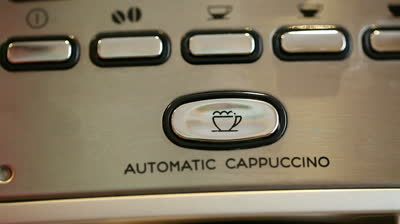
\includegraphics[width=4cm]{media/easy_coffee.jpg}
        \column{.1\textwidth}
            vs.
        \column{.4\textwidth}
            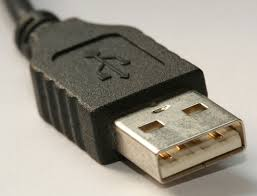
\includegraphics[width=4cm]{media/usb.jpg}
    \end{columns}
}

\frame{
    \frametitle{General usability principles: Visibility}
    \alert{How visible is the state of the system?}
    \vskip30pt
    \begin{columns}
        \column{.4\textwidth}
            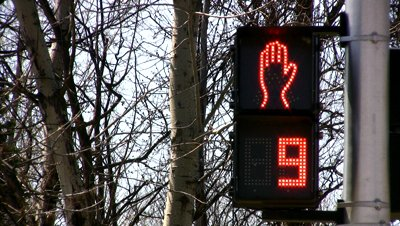
\includegraphics[width=4cm]{media/countdown.jpg}
        \column{.1\textwidth}
            vs.
        \column{.4\textwidth}
            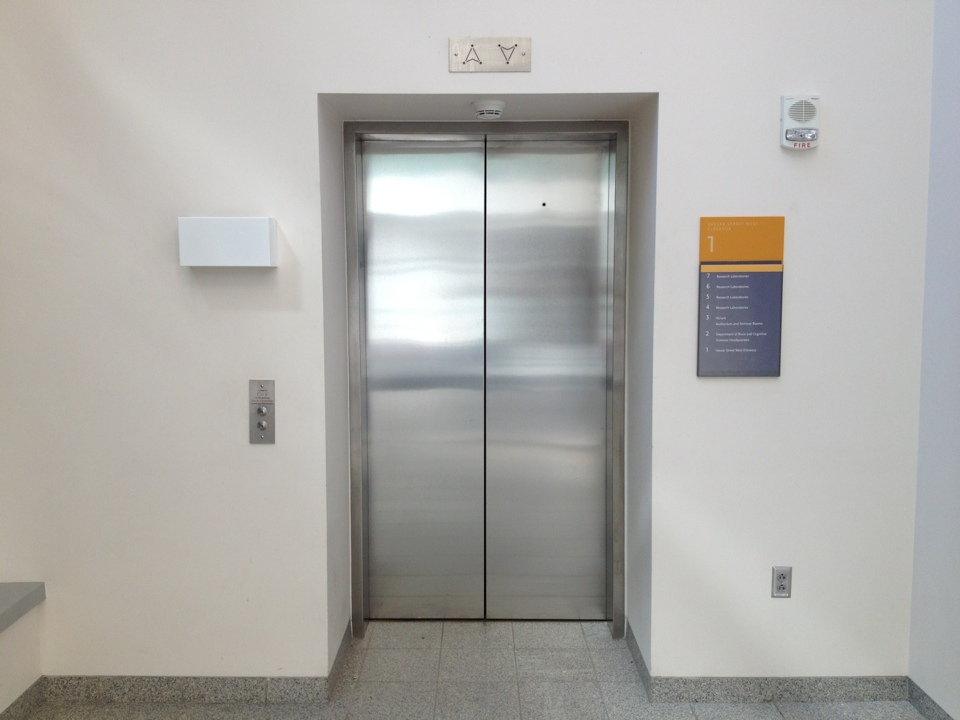
\includegraphics[width=4cm]{media/lift.jpg}
    \end{columns}
}

\frame{
    \frametitle{General usability principles: User control \& memorability}
    \alert{Is user free to explore the system?\\ How easy is it to return to the system after not using it?}
    \vskip30pt
    \begin{columns}
        \column{.45\textwidth}
            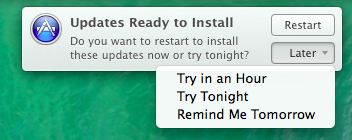
\includegraphics[width=4cm]{media/update.png}
        \column{.1\textwidth}
            vs.
        \column{.45\textwidth}
            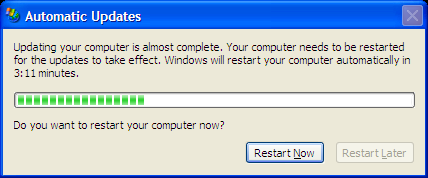
\includegraphics[width=4cm]{media/restart.png}
    \end{columns}
}

\frame{
    \frametitle{General usability principles: Errors}
    \alert{Are errors too easy to make?\\ Are errors easy to recover from?}
    \vskip30pt
    \begin{columns}
        \column{.45\textwidth}
            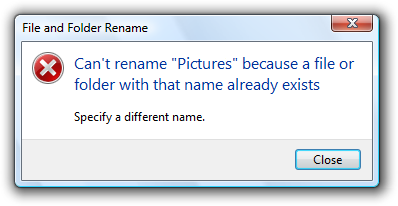
\includegraphics[width=5cm]{media/good_error.png}
        \column{.1\textwidth}
            vs.
        \column{.45\textwidth}
            
\includegraphics[width=5cm]{media/iphone_error.jpg}
    \end{columns}
}   

\frame{
    \frametitle{General usability principles: Efficiency}
    \alert{Once learned, how quickly can tasks be performed?}
}   

\frame{
    \frametitle{General usability principles: Satisfaction}
    \alert{Is the system a pleasure to use?}
    \vskip30pt
    \begin{columns}
        \column{.4\textwidth}
            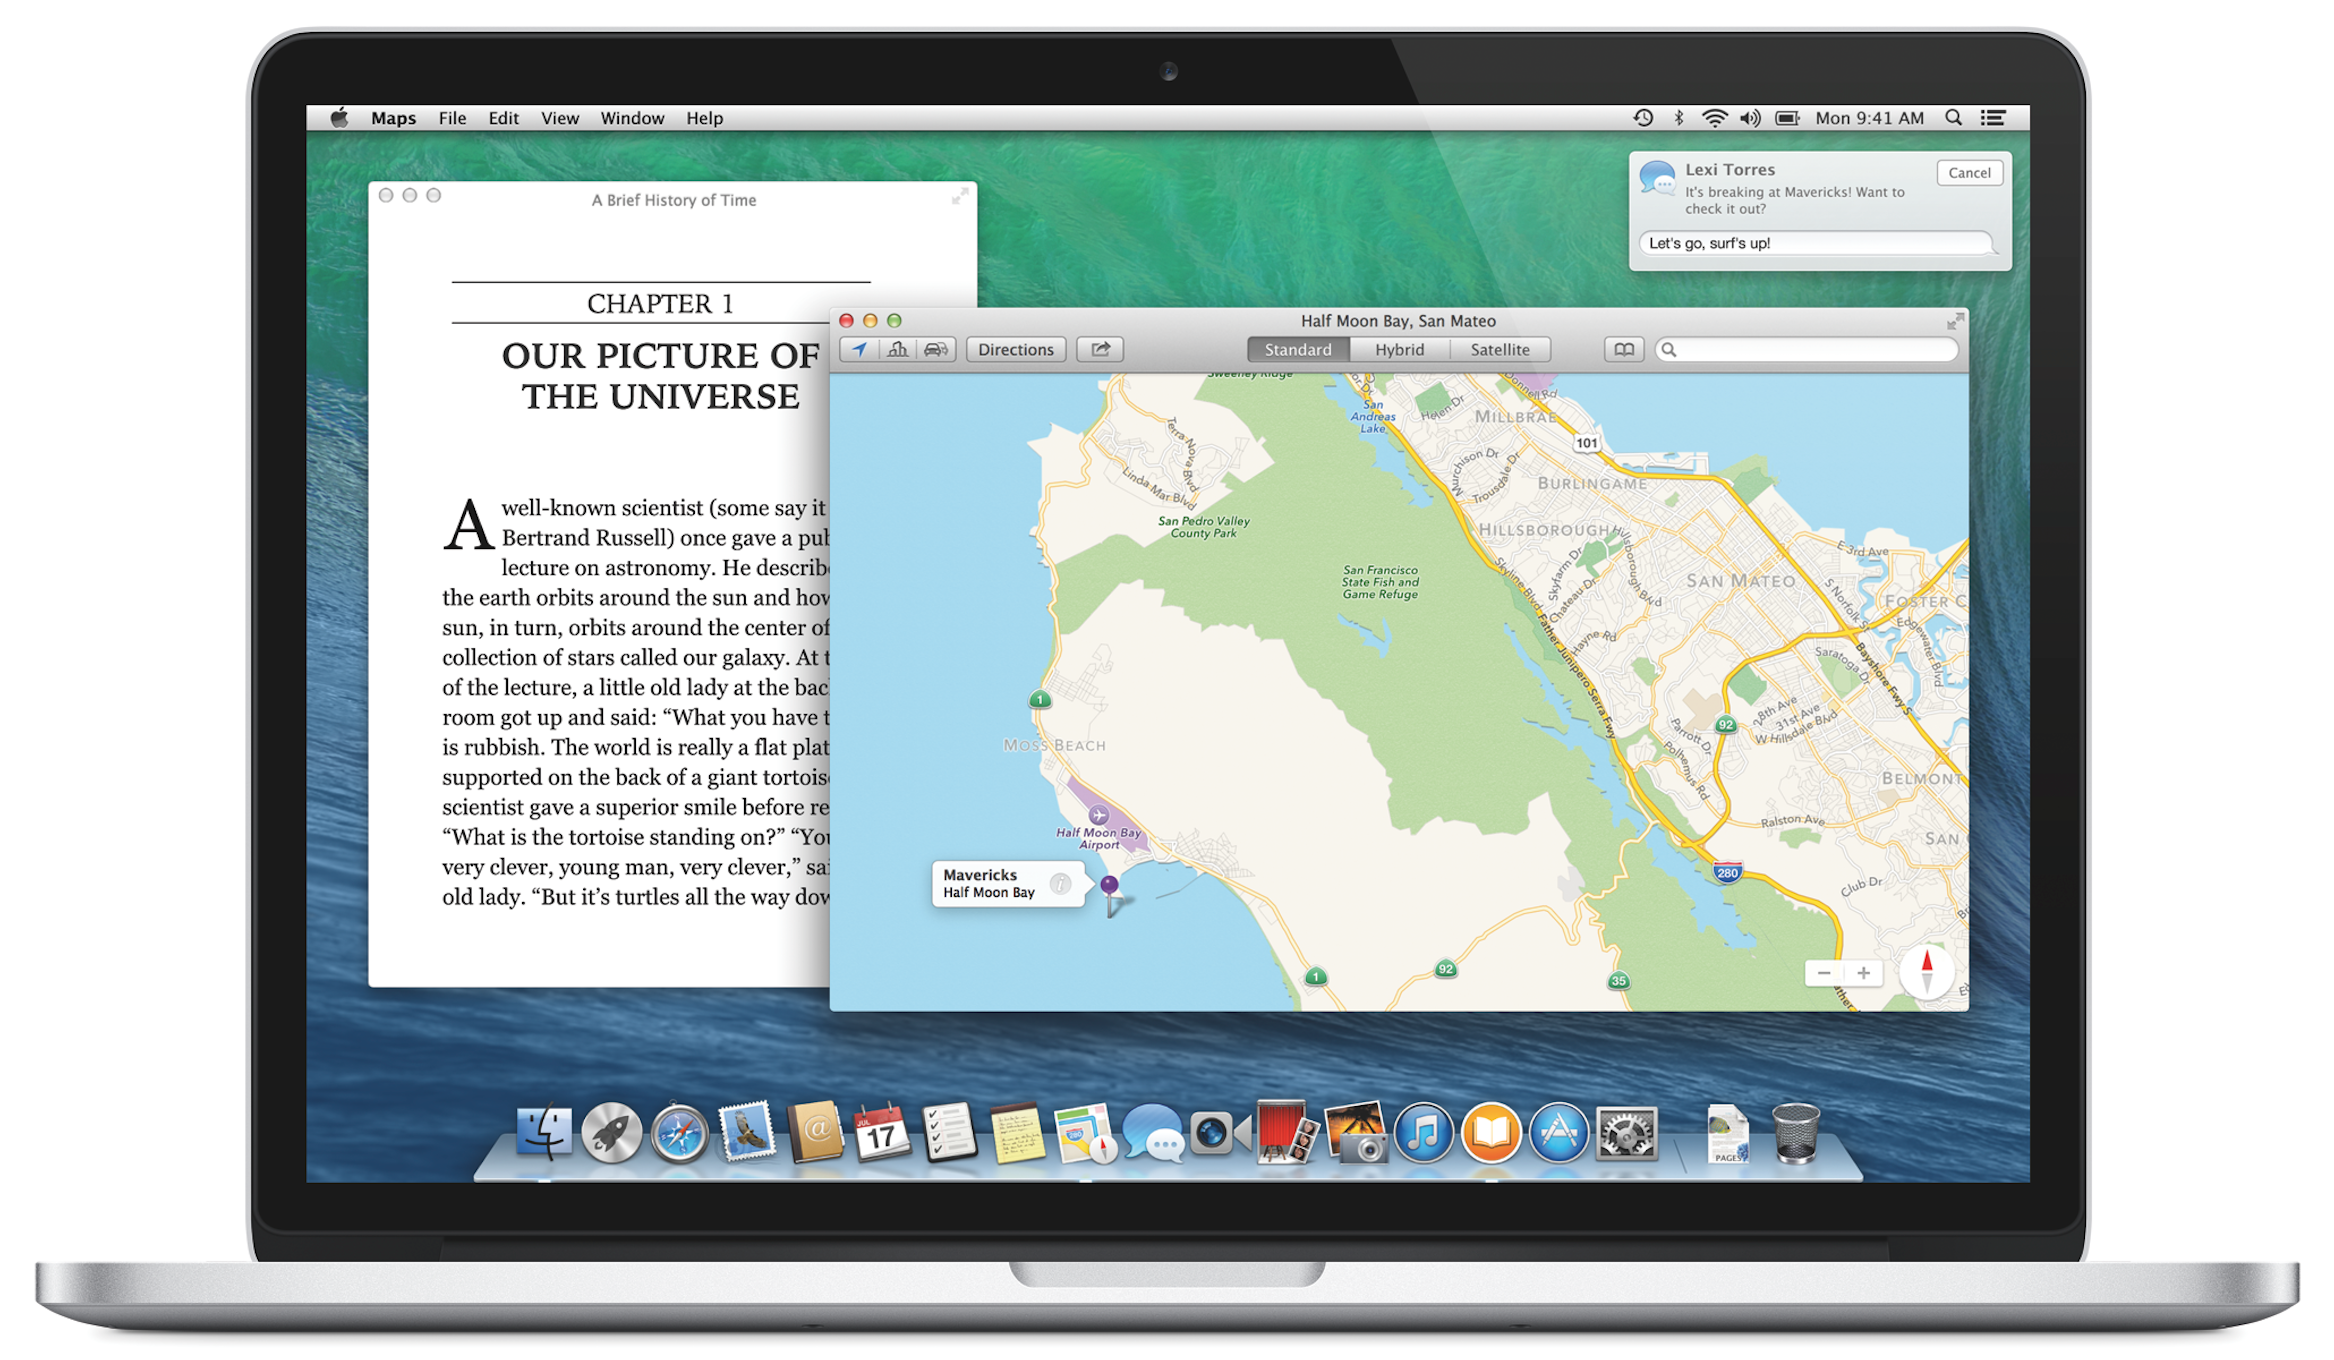
\includegraphics[width=5cm]{media/mavericks.png}
        \column{.1\textwidth}
            vs.
        \column{.4\textwidth}
            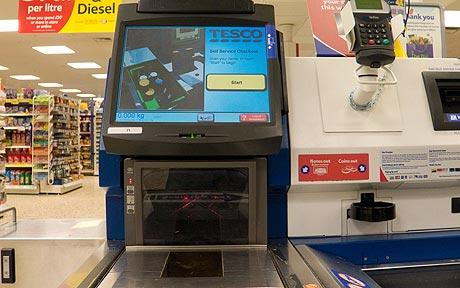
\includegraphics[width=4cm]{media/checkout.jpg}
    \end{columns}
}

\frame{
    \frametitle{General usability principles}
    \begin{itemize}
        \item Systems can be evaluated \alert{with respect to} the principles
        \item When designing interactions, try and \alert{consider all} principles
        \item Aim of systems should be to \alert{maximise} all
    \end{itemize}
    \vskip20pt
    For some systems, some principles are prioritised more than others.\\
    For example, in iOS, \alert{\textit{Satisfaction}} is considered more highly than \alert{\textit{Visibility}}. 
}

\frame{
    \frametitle{General usability principles}
    \center{
        These principles form the baseline for \alert{Neilsen's heuristics}.
    }
    \vskip20pt
    `Heuristics' are broad rules of thumb. Neilsen's heuristics are not specific usability guidelines, but are useful for evaluating systems.
}

\frame{
    \frametitle{Neilsen's heuristics}
    \begin{enumerate}
        \item Visibility of system status
        \begin{itemize}
            \item System should inform users about what's going on internally.
        \end{itemize}
        \item Match between system and real world
        \begin{itemize}
            \item System should speak the user's language and allow functions in a logical order.
        \end{itemize}
        \item User control and freedom
        \begin{itemize}
            \item Provide an `emergency exit' (e.g. by allowing an `undo' action)
        \end{itemize}
        \item Consistency and standards
        \begin{itemize}
            \item Ensure that different words or actions don't mean the same thing. Follow the platform guidelines.
        \end{itemize}
        \item Error prevention
        \begin{itemize}
            \item As well as using good error messages, try and prevent errors from happening.
        \end{itemize}
    \end{enumerate}
}

\frame{
    \frametitle{Neilsen's heuristics}
    \begin{enumerate}
        \setcounter{enumi}{5}
        \item Recognition rather than recall
        \begin{itemize}
            \item Reduce users' memory loads by making actions and options visible. Use standard practices.
        \end{itemize}
        \item Flexibility and efficiency
        \begin{itemize}
            \item Cater to both expert and unexperienced users by making it faster to use for experts.
        \end{itemize}
        \item Aesthetic and minimalist design
        \begin{itemize}
            \item Do not display irrelevant information. Keep interface concise and provice contextually relevant actions.
        \end{itemize}
        \item Help users recognise, diagnose, and recover from errors
        \begin{itemize}
            \item Use English, avoid error codes, constructively provide a solution.
        \end{itemize}
        \item Help and documentation
        \begin{itemize}
            \item If you \textit{do} need documentation, make it easily searchable and task-focussed.
        \end{itemize}
    \end{enumerate}
}


\end{document}
